%!TEX root = ../main.tex

\chapter{Theory}\label{cha:theory}

Many definitions will be now be presented, with the overall aim being to have a rigorous definition for a fingerprint.
Definitions for the Dual, Joss-Ann and Fingerprint were first presented by Ashlock in \cite{Ashlock2004} as mentioned in Section \ref{sec:fingerprinting}.
Then a definition of Finite State Machines will be given, and an explanation of how they relate to fingerprinting.
Finally, an example of how to construct a fingerprint will be shown in Section \ref{sec:analytical-fingerprints}.
In essence this chapter presents a detailed review of the work of
\cite{Ashlock...}  % TODO Grab a bunch of references.

\section{The Joss-Ann}\label{sec:joss-ann}
The Joss-Ann is a basic transformation that can be applied to a strategy.
It operates by making a probabilistic choice of cooperation, defection or the original move.
More formally:

\begin{definition}\label{def:joss-ann}
If $A$ is a strategy for the iterated prisoner's dilemma, then the
\textbf{Joss-Anne of A} denoted by $\JA(A, x, y)$ is a transformation of that strategy.
Instead of the original behaviour, it makes move `C' with probability $x$, move
`D' with probability $y$, and otherwise uses the response appropriate to
strategy $A$ (assuming $x+y < 1$).
\end{definition}

The notation $\JA$ comes from the initials of the names Joss and Anne.
Joss was a strategy submitted to one of Axelrod’s original tournaments and it would occasionally defect without provocation in the hopes of a slight improvement in score.
Anne is the first name of A. Stanley who suggested the addition of random cooperation instead of random defection \cite{Ashlock2008}.
When $x + y = 1$, the original strategy is not used, and the resulting behaviour
is a random strategy with probabilities $(x, y)$. Note that this corresponds to
Random($x$) as described in Section~\ref{ssec:strat_random}.
In more general terms, a $\JA$ strategy is an alteration of $A$ that causes the strategy to be played with random noise inserted into the responses.

\section{The Dual}\label{sec:dual}
The Dual is another, more complex transformation of a strategy (note that both
these transformations can be applied commutatively).

\begin{definition}\label{def:dual}
Strategy $A'$ is said to be the \textbf{Dual} of strategy $A$ if $A$ and $A'$ can be written as finite-state machines that are identical except that their responses are reversed.
\end{definition}

It is important to note that this is different to taking a strategy and flipping its responses.
The dual relies on knowledge of the underlying state of the original strategy, whereas the flip does not.
This is shown in Table \ref{tab:strat-dual-flip}.
For an outline of how Pavlov plays, see Section \ref{ssec:strat_pavlov}.
% TODO Why the pointer to Pavlov here? It's out of place as is.

\section{The Flip}\label{sec:flip}
% TODO This is simpler than the dual, should you present it first?
The Flip is a simple transformation that returns the opposite of the strategy.
This is subtly different from the Dual as demonstrated below.

\begin{definition}\label{def:flip}
Strategy $A'$ is said to be the \textbf{Flip} of strategy $A$ if, $A$ and $A'$ return different actions for the same game history (includes opponent and self).
\end{definition}

\begin{table}[htbp]
    \centering
    \begin{tabular}{l l l l}
        \toprule
        Opponent history & Pavlov & Dual & Flip \\
        \midrule
        C & C & D & D \\
        D & C & D & C \\
        D & D & C & C \\
        C & C & D & C \\
        C & C & D & D \\
        D & C & D & C \\
        C & D & C & C \\
        D & D & C & D \\
          & C & D & D \\
        \bottomrule
    \end{tabular}
    \caption{The different responses of Pavlov, Pavlov's Dual and Flipped Pavlov}
    \label{tab:strat-dual-flip}
\end{table}

The subtle difference between Dual and Flip can be highlighted further by inspecting each row individually.

\underline{Row 1} - Pavlov always plays `C' on the first go.
% TODO More mixing of `C', `C` and $C$. Choose and stick to it.
Flip will change this to `D'.
Dual knows that Pavlov always plays `C' regardless of the opponents history and so swaps to `D'.

\underline{Row 2} - In the previous round for Pavlov the strategies played $(C, C)$, and so Pavlov plays `C' again.
For Flip, the preceding interaction was $(D, C)$, in this instance Pavlov would play `D' again, so this gets flipped to `C'.
The previous turn for Dual was $(D, C)$ so it infers that Pavlov had $(C, C)$.
It knows that Pavlov would play `C' and so plays `D'.

\underline{Row 3} - In the previous round for Pavlov the strategies played $(C, D)$, and so Pavlov would change to play `D'.
For Flip, the preceding interaction was $(C, D)$, in this instance Pavlov would change to `D', so this gets flipped to play `C' again.
The previous turn for Dual was $(D, D)$ so it infers that Pavlov had $(C, D)$.
It knows that Pavlov would play `D' in this instance and so plays `C'.

By following this procedure we can see that the Dual responses and Pavlov's responses are always opposite.
This is achieved by the Dual inferring what the original strategy must have played and then reacting appropriately.
In the above example, Pavlov's memory is only one turn deep, so the Dual only has to infer the preceding turn, however, for more complex strategies, it may need to infer the entire history of the original strategy in order to proceed correctly.

\section{Fingerprint and Double Fingerprint}
The fingerprint function returns the expected score of a strategy when it plays against the Joss-Ann with varying $(x, y)$.
The double fingerprint extends this idea to $x+y \geq 1$.

\begin{definition}\label{def:fingerprint}
A \textbf{Fingerprint} $F_A(S, x, y)$ with $0 \leq x, y \leq 1$, $x+y \leq 1$ for strategy $S$ and \textbf{probe} $A$, is the function that returns the expected score of strategy $S$ against $\JA(A, x, y)$ for each possible $(x, y)$.
\end{definition}

% TODO I think you need to point out that $F_A$ is an analytical expression. So
% a fingerprint is an analytical function. In a way that's very important when
% it comes to probing with strategies that are not representable as FSM. You
% should also include a discussion here about how Ashlock is constrained by
% their choice of probe. Quote something they say about FSM reps.

\begin{definition}\label{def:double-fingerprint}
The \textbf{Double Fingerprint} $F_{AB}(S, x, y)$ with $0 \leq x, y \leq 1$ returns the expected score of strategy $S$ against $\JA(A, x, y)$ if $x+y \leq 1$, and $\JA(B, 1-y, 1-x)$ if $x+y \geq 1$.
\end{definition}

We now show how the double fingerprint, with an appropriate choice of probe, is equivalent to the fingerprint function over the unit square.

\begin{theorem}\label{thm:fingerprint-unit-square}
If $A$ and $A'$ are dual strategies, then $F_{AA'}(S, x, y)$ is identical to the function $F_A(S, x, y)$ extended over the unit square.
\end{theorem}

A proof for this theorem will now be given which was first presented in \cite{Ashlock2004}:
\begin{proof}\label{prf:fingerprint-unit-square}
The Markov chain for the dual strategy $A'$ will have the same transitions as the Markov chain for the strategy $A$.
However, each entry for $x$ corresponds to the probability that the strategy $\JA(A, x, y)$ will randomly choose `C' when it would not normally do so.
For strategy $A'$, this will occur whenever $\JA(A', x, y)$ does not randomly respond `D', which has probability $1 - y$.

Similarly, each $y$ corresponds to the probability that the strategy $\JA(A, x, y)$ will randomly choose `D' when it would usually respond `C'.
For strategy $A'$, this will occur whenever $\JA(A', x, y)$ does not randomly respond `C', which has probability $1 - x$.

Thus the Markov chain for $\JA(A', x, y)$ is the Markov chain for $\JA(A, x, y)$ with the mapping $(x, y) \rightarrow (1-y, 1-x)$.
Therefore $F_{AA'}(S, x, y)$ extends to the remainder of the unit square the function given by $F_A(S, x, y)$. $\blacksquare$
\end{proof}

Theorem \ref{thm:fingerprint-unit-square} allows the fingerprint function to naturally extend over the unit square.
Figure \ref{fig:DualProbe} shows that in the \textcolor{sol-violet}{bottom left} region of the plot, the strategy plays against $\JA(A, x, y)$ and in the \textcolor{sol-cyan}{top right} region it plays against $\JA(A', 1-y, 1-x)$.

\begin{figure}[!hbtp]
    \begin{center}
        \includestandalone{../img/Dual}
        \caption{Where the Strategy plays against the Joss-Ann of the probe or the Joss-Ann of the dual of the probe}\label{fig:DualProbe}
        % TODO Add some labels to this figure: it's just a square with funky
        % colors in.
    \end{center}
\end{figure}

% TODO Introduce the next section and highlight why FSMs are important. Although
% I wonder if you should move the defeinition of an FSM to before your
% definition of a DUAL.
\section{Finite State Machines}\label{sec:fsm}

A formal definition of a Finite State Machine is given by Definition \ref{def:fsm} but first we will outline some motivating key characteristics of a system that can be modelled with a FSM:

\begin{itemize}
 \item The system must be describable by a finite set of states.
 \item The system must have a finite set of inputs that can trigger transitions between states.
 \item The behaviour of the system at a given point in time depends upon the current state and the input that occurs at that time.
 \item For each state the system may be in, behaviour is defined for each possible input.
 \item The system has a particular initial state.
\end{itemize}

We can make the above bullet points rigorous for deterministic cases with the following definition:

\begin{definition}\label{def:fsm}
A \textbf{Deterministic Finite State Machine} $M$ is a tuple $(S, \sigma, \delta, s_0, F)$ where
\begin{itemize}
 \item $\sigma$ is the set of symbols representing the input of $M$.
 \item $S$ is the set of states of $M$.
 \item $s_0 \in S$ is the starting state.
 \item $F \subseteq S$ is the set of final states of $M$.
 \item $\delta: S \times \sigma \rightarrow S$ is the transition function.
\end{itemize}
\end{definition}
%TODO - Add a little paragraph here that shows how this definition matches up with the previous examples.

Figure \ref{fig:Tit4TatFSM} and figure \ref{fig:PavlovFSM} show FSM representations for TitForTat and Pavlov respectively (see Sections \ref{ssec:stra_titfortat} and \ref{ssec:strat_pavlov} for an explanation of how these strategies operate).
Here nodes represent the previous action taken by the strategy and the opponent, ie. node $(D, C)$ implies that on the preceding turn, the strategy chose to Defect and the opponent chose to Co-operate.
Arcs represent the choice made by the opponent at the current turn, and lead us to the state for the next turn.

These are not necessarily the simplest FSM representation of the strategies.
For example, TitForTat requires no knowledge of its own previous moves, but they have been included for completeness.
% TODO It's not just for completeness, if they were omitted than the FSM would not
% indicate to us what TfT does right?

\begin{figure}[hbtp!]
\centering
\subfloat[FSM for TitForTat]{\includestandalone[width = 0.5\textwidth]{../img/Tit4TatFSM}\label{fig:Tit4TatFSM}}
\subfloat[FSM for Pavlov (Win-Stay Lose-Shift)]{\includestandalone[width = 0.5\textwidth]{../img/PavlovFSM}\label{fig:PavlovFSM}}
\\
\subfloat[FSM for Majority in a game with 4 Turns]{\includestandalone[width = 0.8\textwidth]{../img/MajorityFSM}\label{fig:MajorityFSM}}
\caption{Finite State Machine representations for TitForTat, Pavlov and Majority}
\end{figure}

In figure \ref{fig:MajorityFSM} we have a more complex FSM for the strategy Majority for a game with 4 turns.
Majority plays in the following way:

\begin{itemize}
  \item If the opponent has cooperated the majority of the time, Majority will cooperate
  \item If the opponent has defected the majority of the time, Majority will defect
  \item Note - the strategy shown is technically Soft Majority, if the opponents cooperations and defections are equal it will cooperate. Hard Majority would defect in this situation.
\end{itemize}

Clearly this means that the strategy Majority requires knowledge of all previous states.
In general this implies that Majority could not be represented as a FSM.
However if the number of turns in a game is known, any strategy can be represented as a FSM.
% TODO This needs to be stated as a theorem etc.

\section{Proof of FSM for every strategy}\label{sec:fsm_proof}

% TODO


\section{Analytical Fingerprints}\label{sec:analytical-fingerprints}

% TODO This should be before the theorem about FSMs for any strategy.

There are several steps to constructing the Fingerprint of a strategy and basic knowledge of Markov Chains is required.
An outline of the steps is as follows:

\begin{enumerate}
    \item Build a Markov chain model of an IPD between the strategy and probe strategy.
    \item Construct the corresponding transition matrix.
    \item Find the steady state distribution.
    \item Calculate the overall expected score by taking the dot product of the steady state distribution with the payoff vector given in Section \ref{sec:intro_pd} to obtain the fingerprint function.
    \item This can then be plotted as a heat map to make it easier to visualize.
\end{enumerate}

As an example, this process will now be applied to obtain a fingerprint for the strategy Win-Stay-Lose-Shift (sometimes referred to as Pavlov) when probed by Tit-For-Tat.

\textbf{Step 1} - Build the Markov Chain, shown in Figure \ref{fig:PavlovMC}.

\begin{figure}[ht!]
\centering
\includestandalone[width = 0.3\textwidth]{../img/PavlovMarkovChain}
\caption{Markov chain for Pavlov}
\label{fig:PavlovMC}
\end{figure}

\textbf{Step 2} - Construct the transition matrix.

\begin{equation}\label{eq:transition_matrix}
%
T = \bordermatrix{~      & (C, C) & (C, D) & (D, C) & (D, D) \cr
                  (C, C) & 1 - y  & 0      & 0      & x      \cr
                  (C, D) & y      & 0      & 0      & 1 - x  \cr
                  (D, C) & 0      & 1 - y  & x      & 0      \cr
                  (D, D) & 0      & y      & 1 - x  & 0}
%
\end{equation}

\textbf{Step 3} - Find the steady state distribution.

\begin{equation}\label{eq:steady_state}
%
\pi =
\begin{bmatrix}
\cfrac{x (1 - x)}{2y(1-x) + x(1-x) + y(1-y)}, \\
\cfrac{y (1 - x)}{2y(1-x) + x(1-x) + y(1-y)}, \\
\cfrac{y (1 - y)}{2y(1-x) + x(1-x) + y(1-y)}, \\
\cfrac{y (1 - x)}{2y(1-x) + x(1-x) + y(1-y)}
\end{bmatrix}
\end{equation}
\textbf{Step 4} - Calculate the expected score.

\begin{equation}
F = \pi \cdot
\begin{bmatrix}
3 \\
0 \\
5 \\
1
\end{bmatrix}
=
\cfrac{3x(1-x) + y(1-x) + 5y(1-y)}{2y(1-x) + x(1-x) + y(1-y)}
\end{equation}

\textbf{Step 5} - Plot the resulting function, shown in Figure \ref{fig:pavlov_fing_ex}
% TODO This is not technically part of the fingerprinting process. The
% fingerprint is the analytic function.

\begin{figure}[htbp!]
\centering
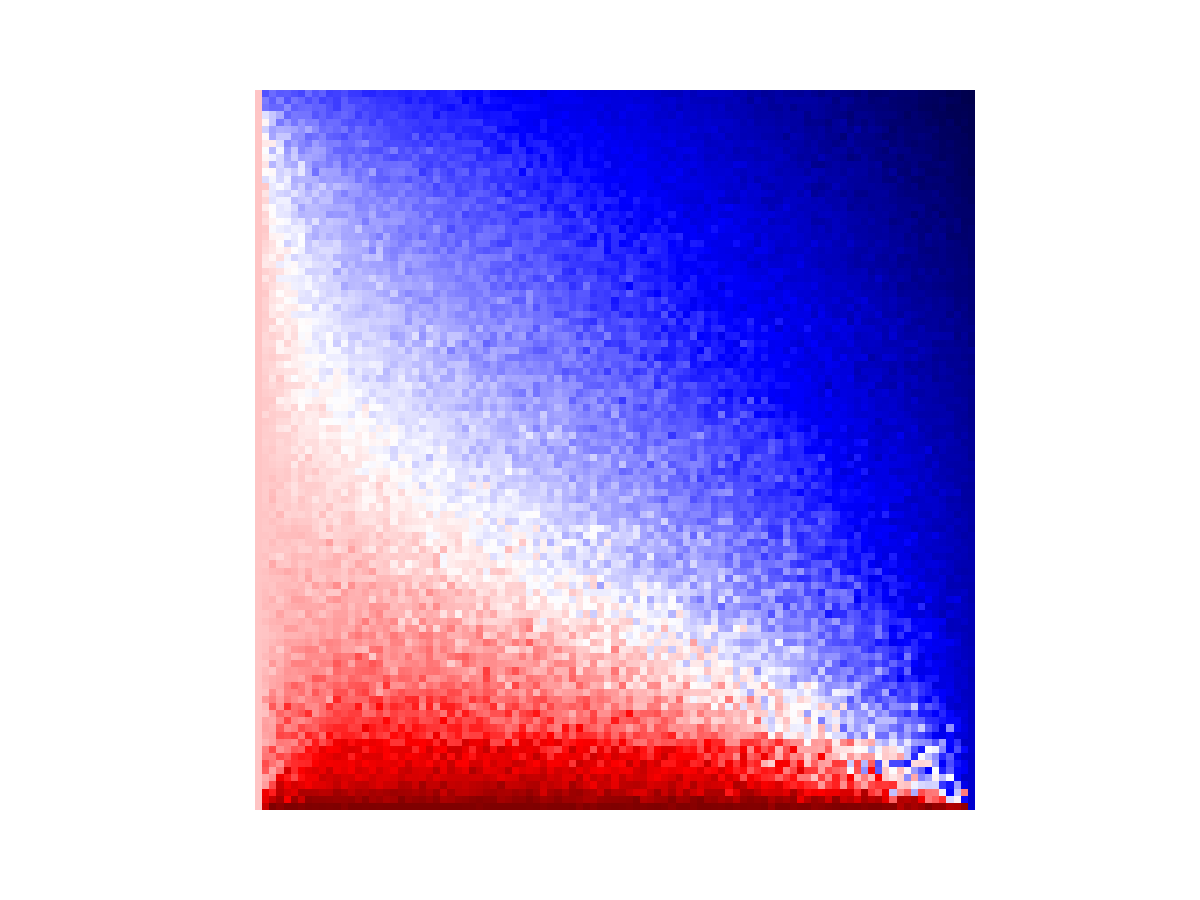
\includegraphics[width = 0.3\textwidth]{../img/Numerical/Win-Stay-Lose-Shift}
\caption{Fingerprint example for Pavlov}
\label{fig:pavlov_fing_ex}
\end{figure}




\begin{theorem}\label{thm:fsm}
Given a deterministic strategy $\alpha$ and 2 histories $h_1, h_2$, then for all games of length $n \in \mathbb{N}$ there exists a FSM such that $\alpha(h_1, h_2)$ can be obtained from the FSM.
\end{theorem}

\begin{proof}\label{prf:fsm}
Let $\sigma = \{C, D\}$ and
\[
S = \bigcup_{i=0}^{n+1} \{C, D\}^i \times \{C, D\}^i
\delta((h_1, h_2), a) =()
\]

\end{proof}

% TODO There is a bit more missing here. The theorem and the fact that we CAN
% probe with any strategy is missed out. You should also point to the relevant
% implementation sections.
% TODO Finally, you also need a conclusion.
